\documentclass[a4paper,12pt]{scrartcl}
\usepackage[utf8]{inputenc}
\usepackage[french]{babel}
\usepackage[T1]{fontenc}
\usepackage{amsmath}
\usepackage{color}
\usepackage{graphicx}
\usepackage{isotope}
\usepackage{float}
\usepackage{scrpage2}
\usepackage{vanadin}
\usepackage[version=3]{mhchem}

  

\title{Résonance magnétique nucléaire (RMN) du \isotope[13]{C} haute résolution en phase solide}
\subtitle{TP Cesire}
\author{Mona Dentler,\\ Sabine Engelhardt et Laura Hilpert}
\publishers{Université Joseph Fourier, CEA Grenoble}

 \begin{document}

\nocite{dokument}

 \pagestyle{empty}
 \begin{center}
  \makeatletter
   %\titlefont
  \@subject
  \vspace{2cm}

  \Huge
  Résonance magnétique nucléaire (RMN) du \isotope[13]{C} haute résolution en phase solide\newline
  \Large TP Cesire
  \vspace{1cm}

  \@author
  \newline\empty\\
  \@publishers


  \@date
  \makeatother
 \end{center}
 \vfill

 \begin{abstract}
  Le but de ce TP Cesire est de comprendre comment faire spectre des solides à l'aide d'une RMN. On le sait déjà très bien faire pour une solution, mais pour un solide il y a quelques problèmes. Un solide est inhomogène et il y a la force dipôlaire qui dérange la mesure, car les atomes sont fortement couplés. En solution cette force se moyenne à zéro.\\ 
  Comment alors obtenir un bon spectre d'un solide? D'abord nous avons appris un peu de la théorie d'une RMN et surtout les solutions pour faire une RMN d'un solide pour ensuite les vérifier en mesurant. 
 \end{abstract}
 \newpage
\pagestyle{scrheadings}
 \tableofcontents

 \section{Résonance Magnétique Nucléaire (RMN)}
  \subsection{Fonctionnement d'une RMN}
  La RMN use la résonance de spin des noyeaux atomiques. L'échantillon est mis dans un champ magnétique $B_0$ externe pour avoir les moments magnétiques des atomes paralell ou anti-paralell au $B_0$. A cause du moment angulaire de l'atome son moment magnétique tourne autour cette direction avec la fréquence de Larmor \\$\omega_L=\frac{\gamma}{2\pi}B_0$, qui est spécifique pour chaque materiél, avec $\gamma$ le rapport gyromagnétique. Le champ magnétique est donc augmenté au direction de $B_0$, mais cette augmentataion est à peine mesurable, car $B_0$ est très grand, alors on use une autre méthode.\\
  Une onde électro-magnétique (em) avec la fréquence $\omega_L$, en grandeur des ondes radio, est envoyé à l'échantillon. Les moments magnétiques commencent à basculer car l'onde em leurs donne l'énergie nécessaire. Normalement on arrêt l'onde quand les spins sont à \unit[90]{\degree} par rapport au $B_o$. Dans cette direction on peut facilement mesurer le champ magnétique $M$, causé par les moments magnétiques, qui se trouve perpendiculaire au $B_0$. \\
  Si on arrête l'onde em, les moments magnétique se remettent en position originale. Cette relaxation est dû à l'interaction spin-spin et à l'interaction de spin-atome. Le temps de relaxation est différent pour chaque matériel et en mesurant le changement de $M$ à l'aide d'une bobine, on peut l'y déduire et ensuite le matériel. Pour ne pas déranger la mesure suivant il faut attendre cet temps pour que les moments magnétiques soient dans la même postition originaire pour ne pas mesurer du bruit.  \newline
  La sensibilité d'une RMN est 
  \begin{equation*}
   \frac{N_{\alpha}}{N_{\beta}}=\exp\left(-\frac{\Delta E}{k\cdot T} \right)=\exp\left(-\frac{\text{h}\nu}{kT}\right)\propto B_0
  \end{equation*}
  donc pour une mesure plus precise on a besoin d'un $B_0$ plus fort et/ou une température de l'échantillon plus basse. Augmenter $B_0$ est très difficile, alors normalement on essaie de froidir l'échantillon. 

  L'atome le plus simple de détecter est l'Hydrogène (H). Cet atome a un moment magnétique très fort, donc il est facile à tourné par l'onde em et son temps de relaxation est assez court ce qui permet de faire des mesures sans un grand retard.

\newpage
  \subsection{RMN d'une solution}
   Avec une dispositif similaire on peut faire un spectre très précise d'une solution à cause de l'isotropie de la solution. Il n'y a pas des défauts causés par des interactions entre les atomes donc on obtient des spectres avec des pics trés précis et larges.

  \subsection{Problématique d'un RMN d'un solide}
   Si on essaie de faire un spectre avec ce dispositif, on ne voit qu'un ou plusieurs signaux très larges et de faible hauteur, alors une distinction entre les atomes ou plutôt les raies du spectre des différents élements n'est pas possible. Ce chevauchement est provoqué par le déplacement chimique causé par les électrons des cortèges électroniques des atomes et par les interactions dipolaires. Cette couplage dipolaire entre les atomes provoque en plus une relaxation assez vite, qui est difficile à mesurer. En outre un solide est anisotrope \c ca veut dire qu'on trouve sous chaque angle un autre ordre des atomes. 

    Le moment magnétique du \isotope[13]{C} est petit, donc on a besoin d'une onde em plus longue pour le basculer pa \unit[90]{\degree} et par conséquence le temps de mesure augmente.

  \subsection{Solutions}
   Car nous avons fait des RMN du \isotope[13]{C}, nous présontons les solution pour cet isotope. Il y a trois aspects différents:
   \begin{enumerate}
    \item La découplage dipolaire pour élimiter les interactions dipolaires.
    \item La rotation à l'angle magique pour éviter l'anisotropie.
    \item La polarisation croisée pour augmenter la sensibilité du \isotope[13]{C}.
   \end{enumerate}

   \subsubsection{Découplage dipolaire}
    Le champ effectif pour le spin d'un atome est
    \begin{equation*}
     B_{eff}=B_0 + B_{couplage} 
    \end{equation*}
    avec $B_{couplage}$ le champ local autour d'atome causé par les interactions dipolaire et scalaires entre les atomes. Par une onde em de haute puissance les couplages entre H et \isotope[13]{C} sont éliminés car l'H est plus sensible que le \isotope[13]{C} et on se  débarasse de l'aimantation $H$ d'H. La découplage est très important pendant le temps de mesure de la relaxation de \isotope[13]{C}. On peut aussi appliquer une impulsion de \unit[90]{\degree} et ensuite changer la phase de l'onde par $\nicefrac{\pi}{2}$ pour garder le moment magnétique perpendiculaire d'H (spin-lock), alors le couplage dipolaire est éliminé. 

   \subsubsection{Rotation de l'angle magique}
    On trouve pour l'aimantation
    \begin{eqnarray*}
     H_{\sigma}&=\hbar H_0\gamma I_z&\left(\frac{1}{2}\sin\left(2\alpha\right)\text{tr}\left(\sigma\right)+\frac{1}{2}\left(3\cos^2\alpha-1\right)\sum_i\sigma_i\sin^2\beta_i\cdot\cos\left(2\left(\omega_r t+\Phi_i\right)\right)\right)\\
     H_{\sigma}\left(t\right)&=\hbar H_0\gamma I_z&\left(\frac{1}{2}\sin\left(2\alpha\right)\sum_i\sigma_i\sin\left(2\beta_i\right)\cos\left(\omega_r t+\Phi_i\right)\right.\\
     &&\left.+\frac{1}{2}\sin^2\alpha \sum_i\sigma_i\sin^2\beta_i\cdot\cos\left(2\left(\omega_r t+\Phi_i\right)\right)\right)
    \end{eqnarray*}
    Avec $\alpha=\unit[54,7]{\degree}$, donc $3\cos^2\alpha-1=0$, entre l'échantillon et $B_0$ on se débarasse du second terme de la première équation. C'est à dire que les interactions dipolaires et quadrupolaires et l'effet de l'anisotropie du déplacement chimique sont éliminés. Une rotation suffisamment vite élimine la dépendance du temps du deuxième équation. Avec une rotation trop lente, il y a plusieurs raies avec une distance égale à la vitesse de la rotation, le raie le plus haute entre eux n'est pas nécessairment le vrai signal. 

   \subsubsection{Polarisation croisée}
    Pour diminuer le temps de mesure on use l'aimantation causépar les moments magnétiques des H pour basculer les moments magnétiques du \isotope[13]{C}. Une impulsion de \unit[90]{\degree} bascule le moment magnétique d'H et après le spin-lock le fixe pour un certain temps. Avec la condition de Hartman-Hahn
    \begin{eqnarray*}
     \omega_C=\omega_H\\
     \Rightarrow \gamma_c H_C=\gamma_H H_H
    \end{eqnarray*}
    l'aimantation est transferé. Le temps de contact pendant laquelle on met la condition Hartman-Hahn doit être ni trop court ni trop long pour obtenir l'aimantation la plus grande pour le \isotope[13]{C}, comme on voit dans la figure \ref{polarisation}. 
    \begin{figure}
     \includegraphics[width=0.6\textwidth]{bilder/schema_pol.png}
     \caption{\label{polarisation} Aimantation de \isotope[13]{C} en fonction du temps de contact}
    \end{figure}
    On y va très bien l'augmentation de l'aimantation perpendiculaire de \isotope[13]{C} à cause de la condition Hartman-Hahn. Après quelque temps l'H se relaxe et donc l'aimantation de \isotope[13]{C} se diminue car moins d'aimantation est transmit et le \isotope[13]{C} se relaxe à son tour.
     

 \section{Dispositif expérimental}
  \subsection{Montage expérimental}
   Nous avons usé deux différents dispositifs expérimentals, leur seule différence est que le deuxième,  celui pour les mesures de la cellulose, donne des résultats plus précises car il est plus neuf.\\
   Chacun des dispositifs se consiste d'un électroaimant pour réaliser le champ magnétique éxterieur $B_0$ dans lequel se trouve l'échantillon. L'échantillon est mis, avec peu d'air pour ne pas obtenir du bruit, dans un petit roteur. Celui est placé dans une bobine, qui se trouve à l'intérieur refroidi du électroaimant. Cette bobine est émetteur et sonde des ondes radios en même temps. Le roteur se tourne sous l'angle magique. \\
   La fréquence de la rotation est choisi directement, la mesure elle-même est dirigé par l'ordinateur, où un logiciel permet de choisir les autres paramètres. Les dates sont directement transferé à l'ordinateur pour donner la possibilté d'y faire une transformation Fourier des dates pour obtenir le spectre.

   Le deuxième dispositif donne la possibilité de mesurer plus précise à cause de deux différence:
   \begin{itemize}
    \item L'intérieur est plus froid, donc le RMN est plus précis
    \item La rotation peut être plus vite à cause d'un roteur plus petit, alors la structure resemble plus homogène
   \end{itemize}


  \subsection{Préliminaire} 
   Pour voir que l'échantillon est bien placé et le dispositif bien calibré, il faut d'abord faire un \flqq wob\frqq. \c Ca veut dire qu'on regarde l'énergie absorbé en fonction de la fréquence. On connaît la fréquence des atomes de l'échantillon, qui on veut mesurer, ici les fréquences du \isotope[13]{C} et de l' H. En envoyant la fréquence sur l'échantillon, on observe, que le système absorbe l'énergie, sauf l'énergie qui correspend à la fréquence qu'on veut mesurer. 

   En ne pas faisant le \flqq wob\frqq avant la mesure, on peut avoir deux problèmes. Premièrement on ne voit rien pendant la mesure, car la réponse, donc la fréquence de la réponse, est absorbé et deuxièment il y a la possibilité que l'énergie pas absorbée est trop grand et détruit la sonde.

   \subsection{Influence des paramètres sur la mesure}
    Les premières mesures, que nous avons fait, avaient pour but de varier les paramètre suivants et voir si la thórie est vraie.
    \subsubsection{Nombre de scans}
     La différence signal/ bruit est proporionnel à $\sqrt{ns}$, donc pour améliorer le résultat par deux il faut avoir un nombre de scans $ns$ 4 fois plus grand.

    \subsubsection{Fréquence de la rotation}
     Si la fréquence est trop petit, on devait obtenir des bandes rotanionelles dans le spectre du distance égale à la fréquence de la rotation. En plus le signal vraie se diminue à cause du nombre de raies plus grand.

    \subsubsection{Temps de contact}
     Comme on a vu dans la figure \ref{polarisation}, il y a une temps de contact optimale. Une temps de contact plus long ou plus court donne des signaux plus petits.

    \subsubsection{Puissance des signaux}
     En changeant la puissance des signaux on change les conditions Hartman-Hahn. Donc l'aimantation des \isotope[13]{C} est moins grand autour de la puissance optimale.

 \section{Glycerine}
  Nous avons fait ces expériment pour verifier les différents aspects présantés pour obtenir le meilleur spectre. Le valeur de départ était déjà le meilleure pour chaque des paramètre. En les changeant nous avons les vérifier.   

  \subsection{Rotation de l'angle magique}
   La première expérience était de changé la fréquence de la rotation de l'angle magique. On a dit que le solide semble plus homogène le plus vite il est tourné. Nous avons fait une mesure avec une rotation à \unit[4]{kHz}, puis \unit[3]{kHz}, \unit[2]{kHz}, \unit[1]{kHz}, \unit[0,75]{kHz}, \unit[0,5]{kHz},\unit[0,2]{kHz} et sans rotation. Dès la mesure de \unit[0,75]{kHz} nous avons augmenté le nombre de scans de 4 à 16 pour obtenir un meilleur spectre. 
   \begin{figure}
   \includegraphics[width=\textwidth]{bilder/rotation.png}
    \includegraphics[width=\textwidth]{bilder/rotation2.png}
    \caption{\label{rotation}Les spectres pour les différents fréquences}
   \end{figure}
   \paragraph{Interprétation}
    On voit bien dans les spectres de la figure \ref{rotation} à la p. \pageref{rotation} que les signaux qu'on veut obtenir se dimunue porportionnelement à la fréquence de la rotation. C'est à cause de la nombre de pics qui augmente. Le même nombre de signaux est detéctés, mais il sont distribue sur différents pics. Dans le premier spectre avec \unit[4]{kHz} on ne voit que les deux pics fines assez grands de $C_1$ et $C_2$. Dans le deuxième spectre on voit déjá plusieurs autres pics, les bandes rotationelles. La distance entre le signal vraie et ses bandes rotationelles est $d=n\cdot f_{rot}$ avec $f_{rot}$ la fréquence de la rotation de l'angle magique. Dans le dernier spectre on ne voit rien. Il n' y a qu'un pic très large avec le maximum même pas à la position correcte. Le deuxième pic, le plus petit, n'est plus vue.

   \paragraph{Conclusion}
    Nous avons vu que les artefacts causé par le déplacement chimique du solide avec la rotation de l'angle magique. En plus une rotation trop lente donne des artefacts, les bandes rotationelles, et diminue le signal vraie.
\pagebreak
  \subsection{Temps de contact}
   Le temps de contact c'est le temps pendant laquelle on transfere l'aimantation de \unit[90]{\degree} des atomes d'H aux atomes de C. Nous avons mesurer 10 différents temps de contact.
   \paragraph{Interprétation}
    Nous avons retrouvé le temps de contact optimal \unit[2]{ns}. En plus nous avons retrouvé la forme attendue de la variation du temps de contact. Le grandeur du signal est proportionel à l'aimentation transferé. L'aimentation $M$ transferé augmente ensuite très vite en augmentant le temps du contact, après un certain temps $M$ se diminue peu à peu à cause de la relaxation. 
    \begin{figure}[H]
     \centering
     \includegraphics[width=0.5\textwidth]{plot/temps.png}
     \caption{Grandeur des raies en fonction du temps de contact}
    \end{figure}
    Les spectres sont presentés dans la figure \ref{temps} à la page \pageref{tatmps}.


   \paragraph{Conclusion}
    Nous avons vu que le temps de contact est important pour obtenir un signal grand. La relation entre le temps de contact et le transfer de l'aimentation est verifié. Nous avons pas suffisamment de points de mesure après le temps idéale pour verifier que le signal se diminue avec le temps de relaxation d'H.
\begin{figure}
    \includegraphics[width=\textwidth]{bilder/figure3.png}
    \includegraphics[width=\textwidth]{bilder/figure4.png}
    \caption{\label{temps} Les spectres pour les différents temps de contact}
   \end{figure}
  \subsection{Puissance de Hartmann-Hahn}
  \todo{Erklärung}
  \paragraph{Interprétation}
  \paragraph{Conclusion}
 \begin{figure}[H]
    \includegraphics[width=\textwidth]{bilder/figure5.png}
  \end{figure}
\begin{figure}[H]
    \includegraphics[width=\textwidth]{bilder/figure6.png}
  \end{figure}
\begin{figure}[H]
 \includegraphics[width=\textwidth]{bilder/figure7.png}
    \caption{Les spectres pour les différents puissances}
   \end{figure}
 

 \section{Graines de salade}
Maintenant nous faisons des spectres des graines de salade. C'est particulièrement	 intéressant, parce qu'il y a une phase liquide et une phase solide dans les graines. On obtient donc des spectres différentes pour l'éxperiment sous condition liquide et pour celui sous conditions adaptées aux échantillons solides.  
  \subsection{Condition liquide}
L'éxperiment à condition liquide montre le spectre suivant: 
 \begin{figurehere}
    \center
    \includegraphics[width=0.5\textwidth]{bilder/graine_liquide.png}
    \caption{graine de salade: condition liquide}
   \end{figurehere}
La phase liquide se compose principalement des lipides et peut-être aussi de l'eau. 
  \subsection{CP/MAS}
Pour obtenir un bon spectre d'un échantillon solide il faut, comme expliqué avant, appliquer quelques conditions spécialles. D'abord nous avons appliquer les conditions CP/MAS \c ca veut dire avec la polarisation croisée et la rotation de l'angle magique. Le séquence de impulsions et le résultat sont donnés ci-dessous.
 \begin{figurehere}
    \center
     \includegraphics[width=0.5\textwidth]{bilder/PDSD1.png}
     \caption{Séquence de la réalisation de \isotope[13]{C} - \isotope[13]{C} dipolaire couplage dans des conditions CP/MAS}
    \end{figurehere}
 \begin{figurehere}
    \center
    \includegraphics[width=0.5\textwidth]{bilder/graine_solide.png}
    \caption{Graines de salade: CP/MAS}
   \end{figurehere}
 \begin{figurehere}
     \begin{minipage}{0.45\textwidth}
      \centering
     \includegraphics[width=\textwidth]{bilder/graine_sans_rot.png}   
     \caption{Graines de salade: sans rotation de l'angle magique}    
   \end{minipage}
   \hfill
   \begin{minipage}[H]{0.45\textwidth}
        \centering
       	\includegraphics[width=\textwidth]{bilder/graine_sans_decouplage.png}
        \caption{Graines de salade: sans découplage}
   \end{minipage}
    \end{figurehere}
  \subsection{DEPT }
Dans l'éxperiment DEPT on transfère la polarisation des protons liés directement à un carbon dans ce-lui. Avec \c ca on peut distinguer entre des carbones avec 1,2,3 ou 4 protons directement liés, c'est-à-dire on va voir les groupes \ce{C-H3}, \ce{C-H2} et \ce{C-H1}. Pour arriver à \c ca, on utilise le séquence suivant, l'aspect le plus important c'est flip angle.  Nous avons realisé une mesure 2D avec DEPT.
\begin{figurehere}
    \center
    \includegraphics[width=0.5\textwidth]{bilder/DEPT.png}
    \caption{sequence DEPT}
   \end{figurehere}  


  \subsection{Spectre 2D}
   On peut aussi appliquer cette technique à 2D (la technique 2D sera expliquée ci-dessous), le \ce{C-H1} va faire deux pics, le \ce{C-H2} trois pics, mais versé à le bas, \ce{C-H3} va faire quatre pics.
  \begin{figurehere}
    \center
    \includegraphics[width=0.5\textwidth]{bilder/dept_2d.png}
    \caption{DEPT 2D}
   \end{figurehere}

\subsection{Conslusion}
\todo{was sieht man daran?}
 

 \section{Cellulose}

  \subsection{Spectre \isotope[13]{C}}
Une première idée pour comprendre la structure de la cellulose, c'est de faire un spectre 1D du carbone. On trouve qu'on peut distinguer le \ce{C1} et le  \ce{C6}, mais pas les autres carbones qui sont présenter par  les pics en centre. Nous avons utilisé les méthodes suivantes pour améliorer notre résultat.
 \begin{figurehere}
    \center
    \includegraphics[width=0.5\textwidth]{bilder/c13_spektum.png}
    \caption{\label{carbon}Spectre du \isotope[13]{C}}
   \end{figurehere}

  \subsection{Spectre H}
Puis nous avons fait un spectre de l'H. On observe juste un vrai pic qui est une superposition des pics différents de l'H, mais encore des bandes rotationelles aux multiples de la fréquence de la rotation. Le pic très fort correspend à l'eau, une liquide, dans l'échantillon.

\begin{figurehere}
    \center
    \includegraphics[width=0.5\textwidth]{bilder/proton_spektrum.png}
    \caption{Spectre d'H avec des artefacts}
   \end{figurehere}
  \subsection{Spin-diffusion}
Comme montré ci-dessus les spectres 1D ne proposent pas toujours une bonne définition des pics. Pour améliorer la distinction tout de même, on ajoute une autre diménsion. Le deuxième dimension découle d'un temps virtuel $t_1$, l'attente après le spin était transferé entre les protons et carbones. Ceux-ci sont decouplés, mais le moment magnétique du carbon se tourne avec le fréquence Lamor. Parce que le détecteur enregistre seulement la part du moment magnétique dans une direction particulière l'amplitude de l'aimantation est modulée sinuso\"{\i}dale. Après on laisse commuter l'aimantation des carbones et finalement on détecte le signal. Au bout du compte il faut faire une deuxième transformation Fourier pour reobtenir le temps $t_1$ codé dans l'amplitude du signal.
\begin{figurehere}
    \center
     \includegraphics[width=0.5\textwidth]{bilder/PDSD2.png}
     \caption{Séquence de réalisation de 2D - \isotope[13]{C} - \isotope[13]{C} dipolaire couplage experiment}
    \end{figurehere}
\begin{figurehere}
    \center
    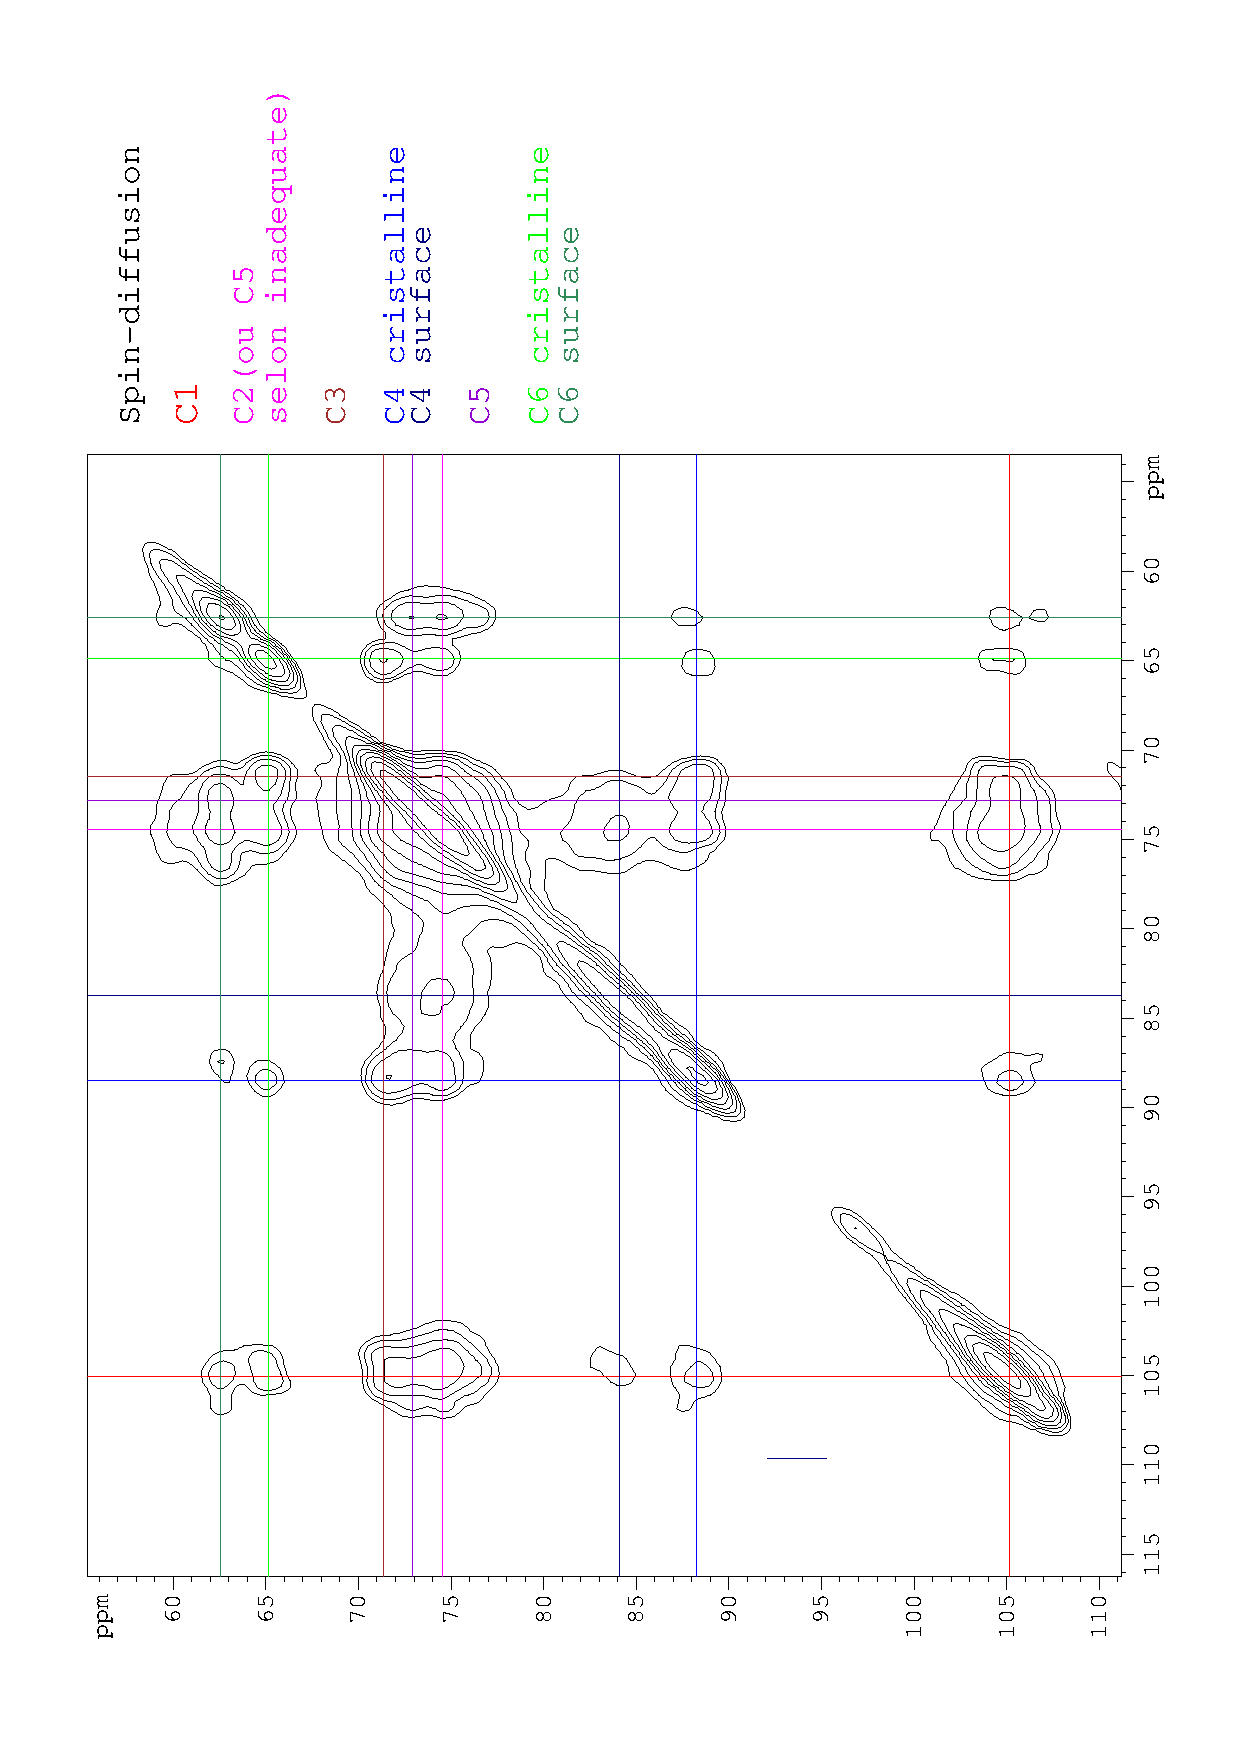
\includegraphics[width=0.5\textwidth]{bilder/spin_diff.png}
    \caption{Proton driven spin-diffusion: \isotope[13]{C} - \isotope[13]{C} dipolaire couplage experiment}
   \end{figurehere}
Dans le spectre \isotope{13}{C} en 1D figure \ref{carbon} nous avons vu les différents pics du carbone dans le cellulose. Il y avait un pic à gauche, le {\ce{C1}, et un pic à droit, le {\ce{C6}, mais on ne peut pas distinguer les pics en centre. A cause de cela nous avons fait une mesure en deux dimensions pour identifier les autres pics. Les pics en diagonale sont les C et les petits crosspeaks à côté de la diagonale montrent les interactions avec les C proches à cause de l’interaction dipolaire. Premièrement nous savons que le premier pic en diagonal chez \unit [105] {ppm} est le \ce{C1}} et le dernier pic en diagonal chez \unit[62,5] {ppm} est le \ce{C6}. Alors nous avons fait des traits horizontals et verticals entre les deux pics pour voir mieux avec quels ils interagissent et pour chaque C que nous avons défini, nous avons fait de nouveau les traits. Nous savons de \cite{dokument} qu’il y a un \ce{C6} cristalline et un \ce{C6} surface pour le \ce{C6} et à cause de cela nous pouvons dire que \ce{C6} surface est chez \unit [22,5] {ppm} et le \ce{C6} cristalline est chez \unit [65] {ppm}. A la prochaine on doit voir avec quels autres carbons le \ce{C6} et le \ce{C1} interagissent selon le spectre. Pour le \ce{C1} on trouve 5 crosspeak et on a une très grande crosspeak qui est probablement l’interaction avec \ce{C5} et \ce{C2} parce que ces deux sont les plus proches. Il faut que ces réfléxions soient fait pour chaque pic en diagonal. En plus nous avons aussi fait la mesure \flqq Inadequate\frqq et avec ce mesure nous pouvons dire un après l'autre quels sont les C en diagonal.  
  
  \subsection{Inadequate}

\begin{figurehere}
    \center
     \includegraphics[width=0.5\textwidth]{bilder/PDSD4.png}
     \caption{Séquence de réalisation de \isotope[13]{C} - \isotope[13]{C} J-couplage experiment}
    \end{figurehere}
Chez la mesure Inadequate nous n’avons pas l’interaction dipolare mais le J couplage. C’est à dire que les crosspeaks qu’on peut voir sont des interactions entre deux C qui on une relation directe. Alors le \ce{C1} a seulement une large crosspeak, mais le \ce{C1} a deux relations directes, une relation avec \ce{C2} et une autre relation avec \ce{C5}. Nous avons cette information de la structure de cellulose \cite{dokument}. Nous ne sommes pas vraiment sûre si la position \unit [74,5] {ppm} correspend à \ce{C5} ou \ce{C2}. On sait que le \ce{C6} a seulement une relation directe avec le \ce{C5} alors on peut dire que le \ce{C5} surface est environ \unit [72,1] {ppm} et le \ce{C5} cristalline est environ \unit [74,9] {ppm}. On peut voir que le \ce{C5} cristalline et le \ce{C2} sont très proches alors il est très difficile de différencer entre les deux. Nous avons comparé la mesure Inadequate avec la mesure spin diffusion et nous avons trouvé les autres C. 
\begin{figurehere}
    \center
    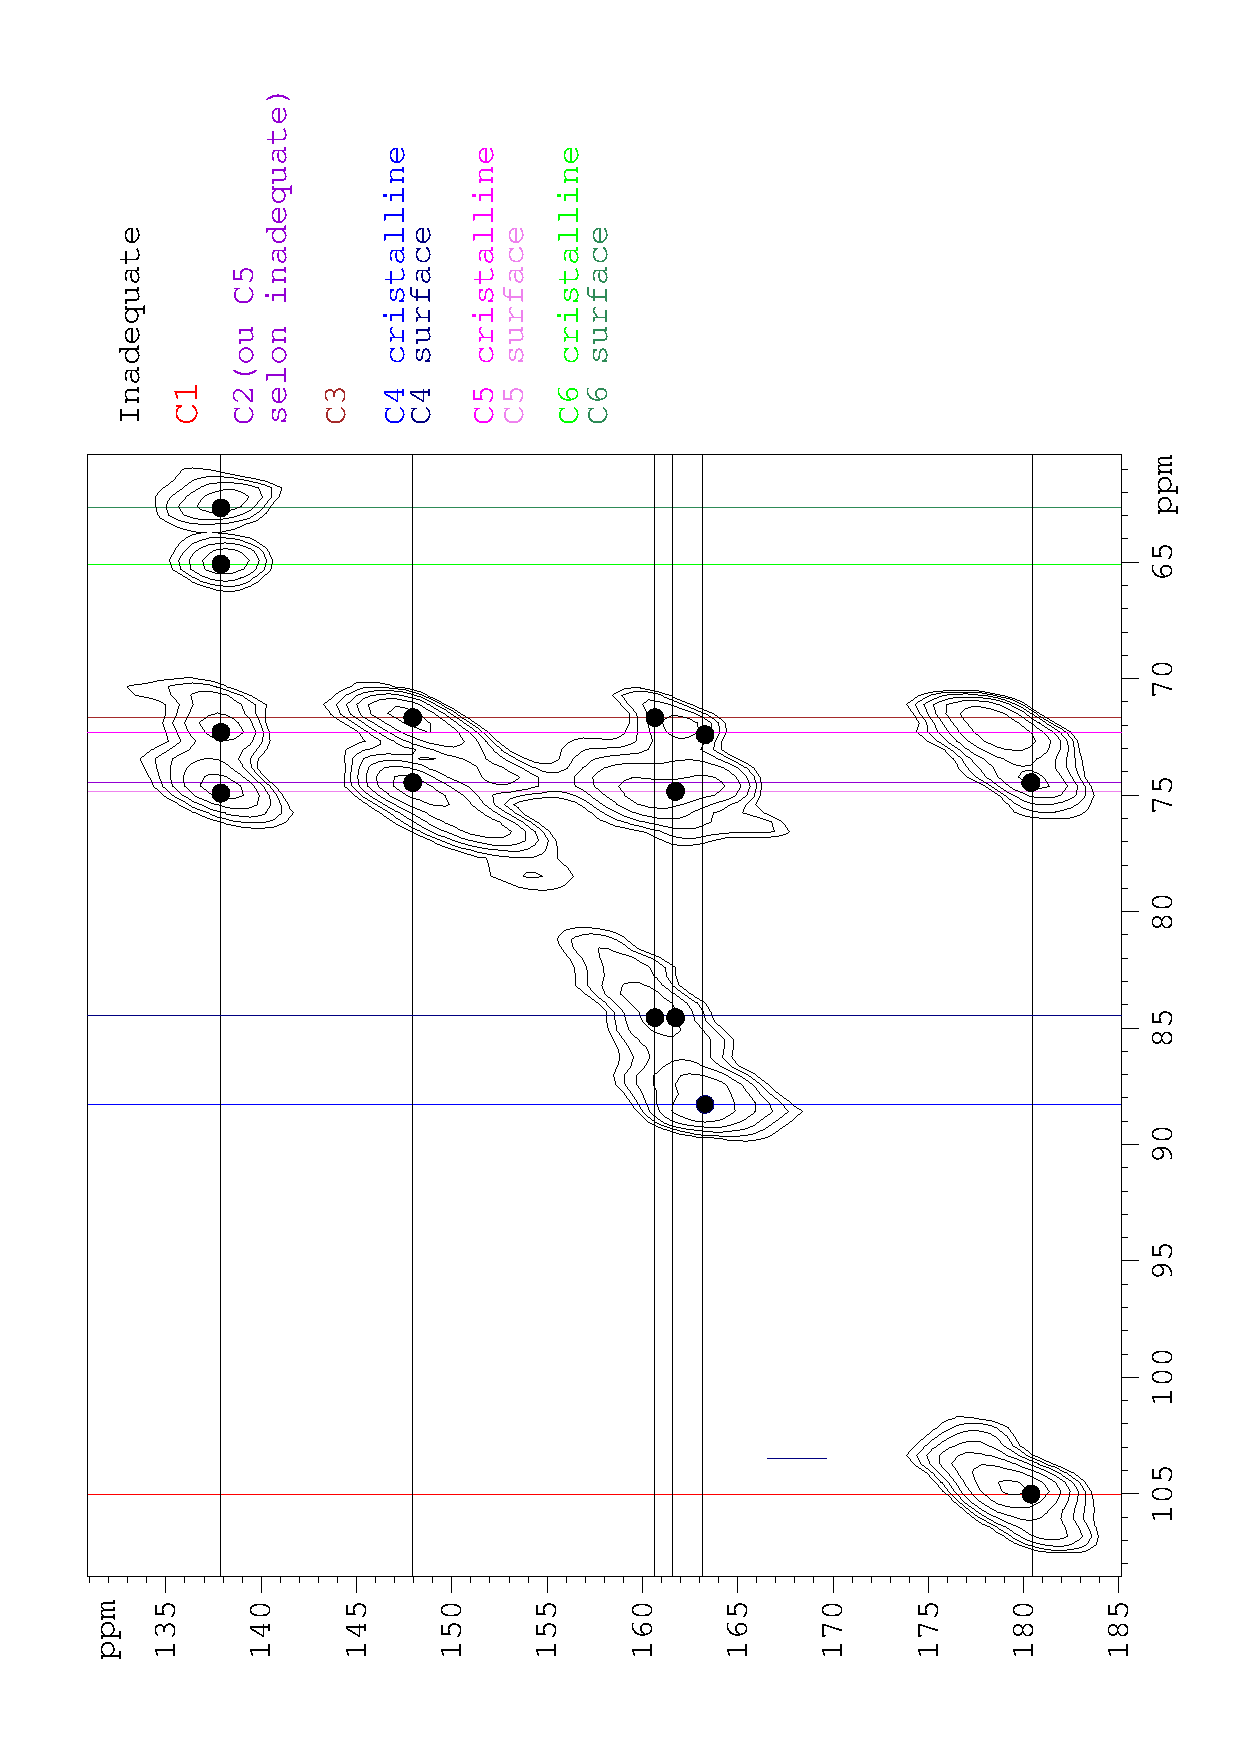
\includegraphics[width=0.5\textwidth]{bilder/inad.png}
    \caption{2D-INADEQUATE: \isotope[13]{C} - \isotope[13]{C} J-couplage }
   \end{figurehere}
  \subsection{Hetcore}
 
  \todo{ abgeschnitten Spinning sidebands, noch da fehler wegen zu kurz gemessen = Signal abgeschnitten???}
\begin{figurehere}
    \center
     \includegraphics[width=0.5\textwidth]{bilder/PDSD3.png}
     \caption{sequence de réalisation de \isotope[1]{H} - \isotope[13]{C} couplage transfert experiment}
    \end{figurehere}
Maintenant nous savons où sont les différents C. En plus nous voulons savoir où les H sont exactement parce que'avec la mesure en 1 dimension nous n'avons reçu qu'un très large pic pur les H. A cause de çela nous avons  aussi fait une mesure avec un couplage \ce{H-C} en 2 dimensions. Nous avons tracé des traits vertical entre les positions des différents pics et aussi des traits horizontals par des pics commons des différents C. On peut dire que le plus grand pic à la position de \ce{C1} est le \ce{H1} et parce qu’il y a aussi deux grands pics au \ce{C6} surface et au \ce{C6} cristalline on peut dire que c’est le \ce{H6}. Nous pouvons voir deux différents pics au \ce{C4} cristalline et au \ce{C4} surface donc nous pouvons dire que c’est le \ce{H4}, mais au \ce{C2}, au \ce{C3} et au \ce{C5}, il y a seulement un grand pic et à cause de çela nous ne pouvons pas dire exactement où sont le \ce{H2}, \ce{H3} et le \ce{H5}.
 \begin{figurehere}
    \center
    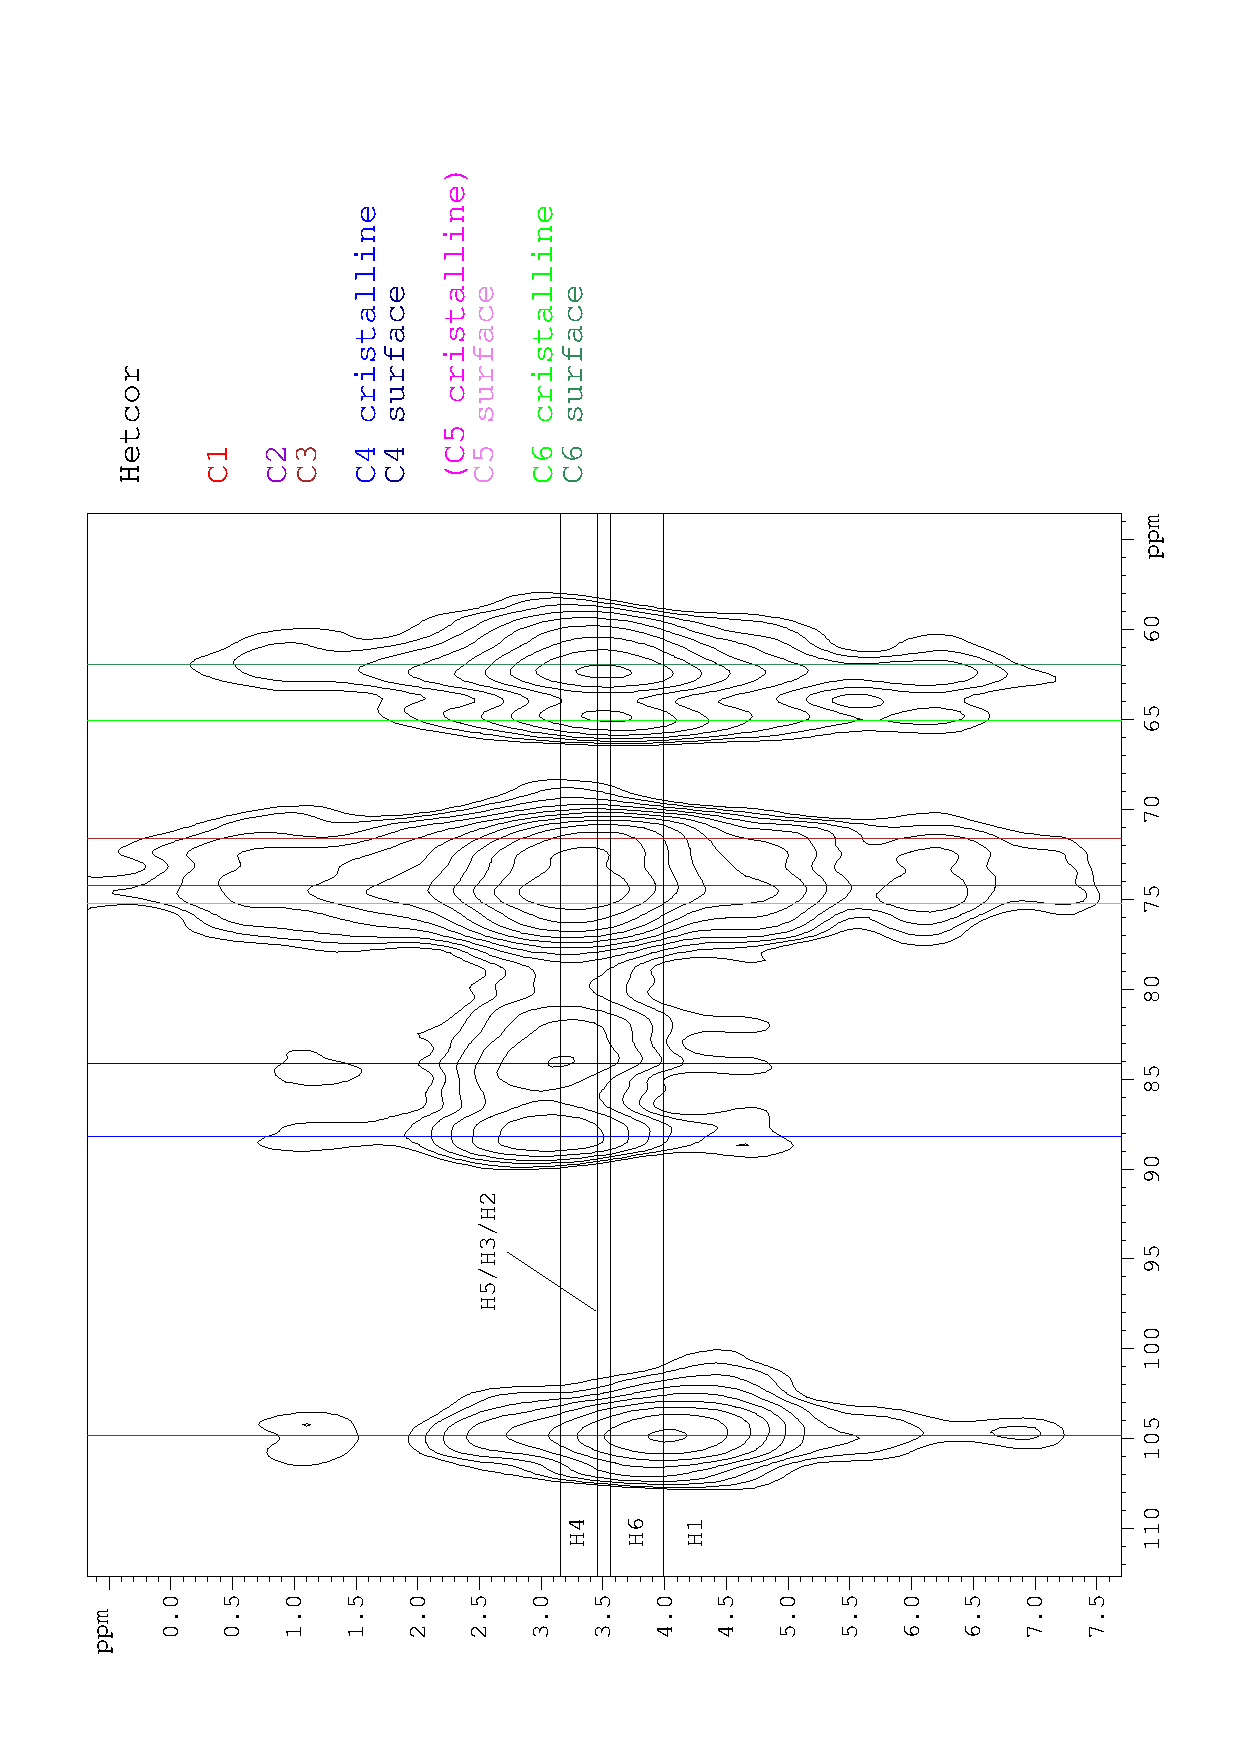
\includegraphics[width=0.5\textwidth]{bilder/hetcor.png}
    \caption{2D-HETCOR: H - \isotope[13]{C} couplage }
   \end{figurehere}
 

 \section{Conclusion}



\bibliographystyle{unsrt}
\bibliography{literatur}
 
 
\listoffigures

\end{document}
